\section{Implementation}\label{sec:implementation}

Talk about how you implemented \lang\ and the general
architecture. Talk about how simple everything is, and also
about how implementing inference for fractions is.

\subsection{Implementation Strategy}

\lang\ transpiles to OCaml and its implementation follows the structure of a
typical domain-specific language (DSL) compiler. Although \lang's current
implementation is not as an embedded DSL, its the general design is simple enough
to adapt to being so and also to target other languages.

Alongside the transpiler, a `Read-Check-Translate' loop, benchmarking program
and a test suite are included in the artifacts accompanying this paper.

\begin{enumerate}

    \item \textbf{Parsing}. A generated, LR(1) parser parses a text file into a
        syntax tree. In general, this part will vary for different languages
        and can also be dealt with using combinators or syntax-extensions (the
        EDSL approach) if the host language offers such support.

    \item \textbf{Desugaring}. The syntax tree is then desugared into a
        smaller, more concise, abstract syntax tree. This allows for the type
        checker to be simpler to specify and easier to implement.

    \item \textbf{Matrix Expressions} are also desugared into the abstract
        syntax tree through some simple pattern-matching.

    \item \textbf{Type checking}. The abstract syntax tree is explicitly typed,
        with some inference to make writing typical programs more convenient.

    \item \textbf{Code Generation}. The abstract syntax tree is translated into
        OCaml, with a few `optimisations' to produce more readable code. This
        process is type-preserving: \lang's type system is embedded into
        OCaml's (Figure~\ref{fig:type_grammar}), and so the OCaml type checker
        acts as a sanity check on the generated code.

\end{enumerate}

A very pleasant way to use \lang\ is to have the build system generate code at
\emph{compile-time} and then have the generated code be used by other modules
like normal OCaml functions. This makes it possible and even easy to use \lang\
alongside existing OCaml libraries; in fact, this is exactly how the
benchmarking program and test-suite use code written in \lang.

\subsubsection{Desugaring, Matrix Expressions and Type Checking}\label{subsubsec:initial}

Desugaring is conventional, outlined in Figure~\ref{fig:lang_desugar}.  Matrix
expression are translated into BLAS/ LAPACK calls via purely syntactic
pattern-matching, outlined in Figure~\ref{fig:lang_matexp}. Type checking is
mostly standard for a linearly typed language, with the exception of fractional
permission inference.  Because all functions must have their argument types
explicitly annotated, inferring the correct fraction at a call-site is simply a
matter of unification.

\textsc{What more can/should we say here?}

\begin{figure}[t]
\begin{center}
\[\def\arraystretch{1.3}
    \begin{array}{rcl}
    x[e] &
    \Rightarrow &
    \mathbf{get}\ \_\ x\ (e) \;\qquad \textrm{(similarly for matrices)}
\\
    x[e_1] := e_2 &
    \Rightarrow &
    \mathbf{set}\ x\ (e_1)\ (e_2) \quad \textrm{(similarly for matrices)}
\\
\\
    pat & ::= & ()\ \mid\ x\ \mid\ !x\ \mid\ \mathbf{Many\ } pat\ \mid\ (pat, pat)
\\
    \mathbf{let}\ !x = e_1\ \mathbf{in}\ e_2 &
    \Rightarrow &
    \specialcell[t]{l}{\mathbf{let\ Many}\ x = e_1\ \mathbf{in\ } \\
    \mathbf{let\ Many}\ x = \mathbf{Many}\ (\mathbf{Many}\ x)\ \mathbf{in}\ e_2}
\\
    \mathbf{let\ Many} \langle pat_x \rangle\ = e_1\ \mathbf{in}\ e_2 &
    \Rightarrow &
    \specialcell[t]{l}{%
        \mathbf{let\ Many}\ x = x\ \mathbf{in\ } \\
        \mathbf{let\ }\ \langle pat_x \rangle\ = x\ \mathbf{in\ } e_2}
\\
    \mathbf{let}\ (\langle pat_a \rangle, \langle pat_b \rangle)\  = e_1\ \mathbf{in}\ e_2 &
    \Rightarrow &
    \specialcell[t]{l}{%
        \mathbf{let\ }\ (a,b)\ = a\_b\ \mathbf{in\ }
        \ \mathbf{let\ }\ \langle pat_a \rangle\ = a\ \mathbf{in\ } \\
        \mathbf{let\ }\ \langle pat_b \rangle\ = b\ \mathbf{in\ } e_2}
\\
    \mathbf{fun}\ (\langle pat_x \rangle\ : t) \rightarrow e &
    \Rightarrow &
    \mathbf{fun}\ (x : t) \rightarrow \mathbf{let\ }\ \langle pat_x \rangle = x\ \mathbf{in\ } e
\\
\\
    arg & ::= & \langle pat \rangle : t\ \mid\ {'x} \textrm{ (fractional permission variable)}
\\
    \mathbf{fun}\ \langle arg_{1 .. n} \rangle \rightarrow e &
    \Rightarrow &
    \mathbf{fun}\ \langle arg_1 \rangle \rightarrow ..
    \ \mathbf{fun}\ \langle arg_n \rangle \rightarrow e
\\
    \mathbf{let}\ f\ {\langle arg_{1 .. n} \rangle} = e_1\ \mathbf{in}\ e_2 &
    \Rightarrow &
    \mathbf{let}\ f = \mathbf{fun}\ {\langle arg_{1 .. n} \rangle} \rightarrow e_1\
    \mathbf{in}\ e_2
\\
    \mathbf{let}\ f\ {\langle arg_{1 .. n} \rangle} = e_1\ \mathbf{in}\ e_2 &
    \Rightarrow &
    \mathbf{let}\ f = \mathbf{fun}\ {\langle arg_{1 .. n} \rangle} \rightarrow e_1\
    \mathbf{in}\ e_2
\\
    \mathbf{let}\ !f\ {\langle arg_{1 .. n} \rangle} = e_1\ \mathbf{in}\ e_2 &
    \Rightarrow &
    \mathbf{let\ Many}\ f = \mathbf{Many}\ (\mathbf{fun}\ {\langle arg_{1 .. n} \rangle}
    \rightarrow e_1)\ \mathbf{in}\ e_2
\\
    \mathbf{let\ rec}\ f\ (x : t)\ {\langle arg_{1 .. n} \rangle} : {t'} = e_1\ \mathbf{in}\ e_2 &
    \Rightarrow &
    \specialcell[t]{l}{\mathrm{fixpoint} \equiv \mathbf{fix}\ (f, x : t,
        \mathbf{fun}\ {\langle arg_{1 .. n} \rangle} \rightarrow e_1 : {t'} ) \\
    \mathbf{let\ Many}\ f = \mathbf{Many}\ \mathrm{fixpoint}\ \mathbf{in}\ e_2}
    \end{array}
\]
\end{center}
\caption{Desugaring from \lang\ concrete syntax to core constructs.}\label{fig:lang_desugar}
\end{figure}

\begin{figure}[t]
\begin{center}
\[\def\arraystretch{1.3}
    \begin{array}{rcl}
    \mathbf{let\ } v \leftarrow x[e]\ \mathbf{in\ } e &
    \Rightarrow &
    \mathbf{let\ } (x, !v)\ = x[e]\ \mathbf{in\ } e \qquad \textrm{(similarly for matrices)}
\\
    \mathbf{let\ } x_2 \leftarrow \mathbf{new}\ [|\ x_1\ |]\ \mathbf{in\ } e &
    \Rightarrow &
    \mathbf{let\ } (x_1, x_2)\ = \mathbf{copyM\ } \_\ x_1\ \mathbf{in\ } e
\\
    \mathbf{let\ } x_2 \leftarrow [|\ x_1\ |]\ \mathbf{in\ } e &
    \Rightarrow &
    \mathbf{let\ } (x_1, x_2)\ = \mathbf{copyM\_to\ } \_\  x_1\ x_2\ \mathbf{in\ } e
    \end{array}
\]
\[
    M ::= X\ \mid\ X^T\ \mid\ \textrm{sym}( X )
\]
\end{center}
\begin{align*}
% new
    \mathbf{let\ } &Y \leftarrow \mathbf{new}\ (n, k)\ [|\ \alpha M_1 M_2 \ |]\ \mathbf{in\ } e
    \Rightarrow \\
    & \mathbf{let\ } Y\ = \mathbf{matrix\ } n\ k\ \mathbf{in}
    \ \mathbf{let\ } Y \leftarrow [|\ \alpha M_1 M_2 + 0Y\ |]\ \mathbf{in\ } e \\
\\
%syrk
    \mathbf{let\ } &Y \leftarrow [|\ \alpha X X^T + \beta Y\ |]\ \mathbf{in\ } e
    \Rightarrow \\
    & \mathbf{let\ } (X,Y)\ = \mathbf{syrk\ } \mathbf{false}
    \ \alpha\ \_\ X\ \beta\ Y\ \mathbf{in\ } e \\
\\
    \mathbf{let\ } &Y \leftarrow [|\ \alpha X^T X + \beta Y\ |]\ \mathbf{in\ } e
    \Rightarrow \\
    & \mathbf{let\ } (X,Y)\ = \mathbf{syrk\ } \mathbf{true}
    \ \alpha\ \_\ X\ \beta\ Y\ \mathbf{in\ } e \\
%symm
\\
    \mathbf{let\ } &Y \leftarrow\ [|\ \alpha\,\textrm{sym}(X_1)\,X_2 + \beta Y\ |]\ \mathbf{in\ } e
    \Rightarrow \\
    & \mathbf{let\ } ((X_1,X_2),Y)\ = \mathbf{symm\ } \mathbf{false}
        \ \alpha\ \_ \ X_1 \_\ X_2\ \beta\ Y\ \mathbf{in\ }e \\
\\
    \mathbf{let\ } &Y \leftarrow\ [|\ \alpha\,X_2\,\textrm{sym}(X_1) + \beta Y\ |]\ \mathbf{in\ } e
    \Rightarrow \\
    & \mathbf{let\ } ((X_1,X_2),Y)\ = \mathbf{symm\ } \mathbf{false}
        \ \alpha\ \_ \ X_1 \_\ X_2\ \beta\ Y\ \mathbf{in\ } e \\
\\
%gemm
    \mathbf{let\ } &Y \leftarrow [|\ \alpha X_1^{T?} X_2^{T?} + \beta Y\ |]\ \mathbf{in\ } e
    \Rightarrow \\
    & \mathbf{let\ } ((X_1,X_2),Y)\ =\ \mathbf{gemm\ } \alpha
        \ \_\ \left(X_1, \substack{\mathbf{true}\\\mathbf{false}}\right)
        \ \_\ \left(X_2, \substack{\mathbf{true}\\\mathbf{false}}\right)
        \ \beta\ Y\ \mathbf{in\ } e
\end{align*}

\caption{Purely syntactic pattern-matching translations of
    matrix expressions.}\label{fig:lang_matexp}
\end{figure}

\subsubsection{Code Generation} is a straightforward mapping from \lang's core
constructs to high-level OCaml ones. We embed \lang's type- and term-
constructors into OCaml as a sanity check on the output
(Figure~\ref{fig:type_grammar}).

\begin{figure}[t]
    \centering
    \begin{minipage}{.3\textwidth}
        \centering
        \begin{grammar}
            <f> ::= `'
            \alt <fc>
            \alt `Z'
            \alt `S' <f>

            <t> ::= `'
            \alt `unit'
            \alt `bool'
            \alt `int'
            \alt `elt'
            \alt <f> `arr'
            \alt <f> `mat'
            \alt `!' <t>
            \alt \synt{$\forall$} <fc.> <t>
            \alt <t> \lit{$\otimes$} \synt{$t'$}
            \alt <t> \lit{$\multimap$} \synt{$t'$}
        \end{grammar}
    \end{minipage}
    \begin{minipage}{.3\textwidth}
        \centering
        \begin{minted}[fontsize=\small]{ocaml}
module Arr =
  Owl.Dense.Ndarray.D

type z = Z
type 'a s = Succ

type 'a arr =
  A of Arr.arr
  [@@unboxed]

type 'a mat =
  M of Arr.arr
  [@@unboxed]

type 'a bang =
  Many of 'a
  [@@unboxed]
        \end{minted}
    \end{minipage}
    \begin{minipage}{.3\textwidth}
        \begin{align*}
            [\![ f\!c ]\!] &= \texttt{'fc} \\
            [\![ \textbf{Z} ]\!] &= \texttt{z}\\
            [\![ \textbf{S} \, f ]\!] &= [\![ f ]\!]\, \texttt{s}\\
            [\![ \textbf{unit} ]\!] &= \texttt{unit}\\
            [\![ \textbf{bool} ]\!] &= \texttt{bool}\\
            [\![ \textbf{int} ]\!] &= \texttt{int}\\
            [\![ \textbf{elt} ]\!] &= \texttt{float}\\
            [\![ f\, \textbf{arr} ]\!] &= [\![ f ]\!]\, \texttt{arr}\\
            [\![ f\, \textbf{mat} ]\!] &= [\![ f ]\!]\, \texttt{mat}\\
            [\![ \textbf{!} \, t ]\!] &= [\![ t ]\!]\, \texttt{bang}\\
            [\![ \forall f\!c.\, t ]\!] &= [\![ t ]\!]\\
            [\![ t \otimes t' ]\!] &= [\![ t ]\!] \texttt{*} [\![ t' ]\!]\\
            [\![ t \multimap t' ]\!] &= [\![ t ]\!] \rightarrow [\![ t' ]\!]
        \end{align*}
    \end{minipage}
    \caption{\lang's type grammar (left) and its embedding into OCaml
        (right).}\label{fig:type_grammar}
\end{figure}

This is also useful when using \lang\ from within OCaml; for example, we can
use existing tools to inspect the type of the function we are using
(Figure~\ref{fig:build}). It is worth reiterating that only the type- and term-
constructors are translated into OCaml, \lang's precise control over linearity
and aliasing are not brought over.

We actually use this fact to our advantage to clean up the output code by
removing what would otherwise be redundant re-bindings in the output OCaml.
Combined with a code-formatter, the resulting code is not obviously correct and
exactly what a programmer would intend to write by hand, but now with the
guarantees and safety of \lang\ behind it.

\begin{figure}[t]
    \centering
    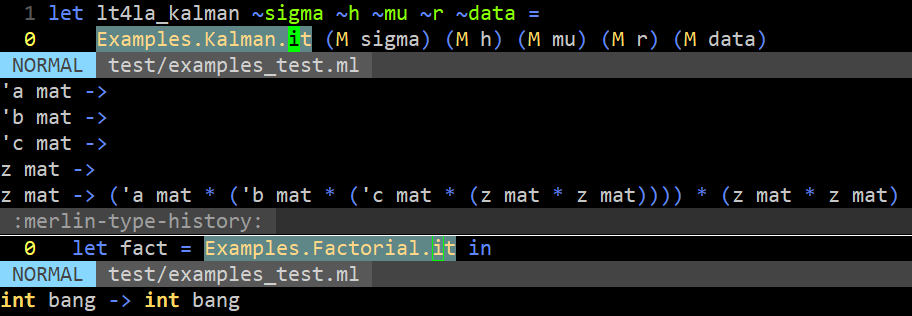
\includegraphics[width=\textwidth]{impl_build}
    \caption{Using \lang\ functions from OCaml.}\label{fig:build}
\end{figure}

A few examples?

\subsection{Performance Metrics}

Here, evaluate the performance of the examples from the second
section.  Compare with your C implementations, and perhaps as well as
the straightforward math transcribed into (Matlab/R/Numpy?).
